\chapter{Grayscale}

To convert an image to gray scale three channels needs to be converted to one channel. The remaining channel needs to capture a kind of mean of the other channels. This can be done with different formulars. It is possible to use luminosity formular $ 0.21r + 0.72g + 0.07b $. But this project uses the same formular like OpenCV uses, $ 0.299r + 0.587g + 0.114b $, to make results better comparable.

\section{Performance Tests}

As shown in the figure bellow, all implementations perform between an image conversion between $ 4 $ ms and $ 45 $ ms. Best performance is delivered by using at least 4 threads. Using more threads doesn't result in a significant performance boost. With more than 8 threads the performance drops significantly parallelizing the inner For-Loop. In general parallelization on the outer For-Loop works best.

\begin{center}
    \begin{figure}[H]
        \centering

        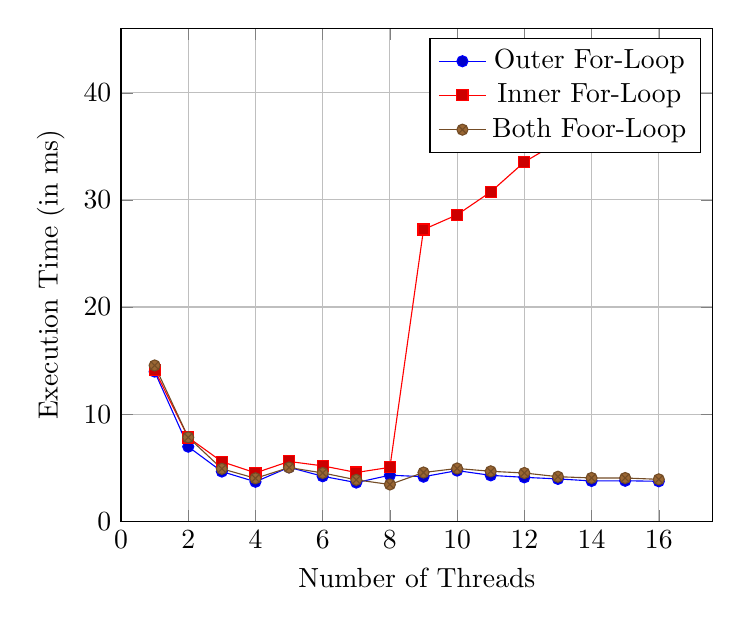
\begin{tikzpicture}
            \begin{axis}[
                title={},
                width=0.75\textwidth,
                xlabel={Number of Threads},
                ylabel={Execution Time (in ms)},
                xmin=0,
                ymin=0,
                grid=major
            ]
                \addplot coordinates {
                    (1,13.9745)(2,6.96595)(3,4.6442)(4,3.68995)(5,5.03995)(6,4.20395)(7,3.61295)(8,4.3057)(9,4.1637)(10,4.7335)(11,4.28995)(12,4.10465)(13,3.9569)(14,3.76905)(15,3.7839)(16,3.7353)
                };
                \addlegendentry{Outer For-Loop}

                \addplot coordinates {
                    (1,14.1323)(2,7.823)(3,5.5688)(4,4.5187)(5,5.58615)(6,5.1761)(7,4.5574)(8,5.0374)(9,27.2378)(10,28.6125)(11,30.7489)(12,33.5384)(13,35.3871)(14,36.3363)(15,39.2266)(16,41.8422)
                };
                \addlegendentry{Inner For-Loop}       

                \addplot coordinates {
                    (1,14.5495)(2,7.8367)(3,4.9025)(4,4.01435)(5,5.0195)(6,4.5141)(7,3.8719)(8,3.4367)(9,4.55745)(10,4.93435)(11,4.66755)(12,4.50995)(13,4.16325)(14,4.048)(15,4.0425)(16,3.9195)
                };
                \addlegendentry{Both Foor-Loop}
            \end{axis}
        \end{tikzpicture}
        \caption{Grayscale Performance Tests}
    \end{figure}
\end{center}

\section{Results}

Using the same formular like OpenCV yields the exactly the same results. Subtracting the two resulting image matrices equals to $ 0 $.

\begin{figure}[H]
    \centering

    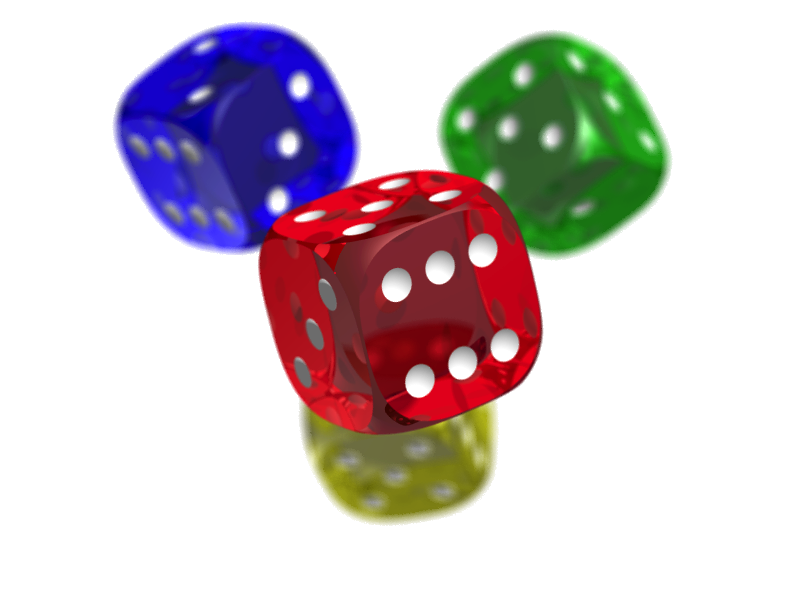
\includegraphics[width=0.20\textwidth]{images/dice.png}
    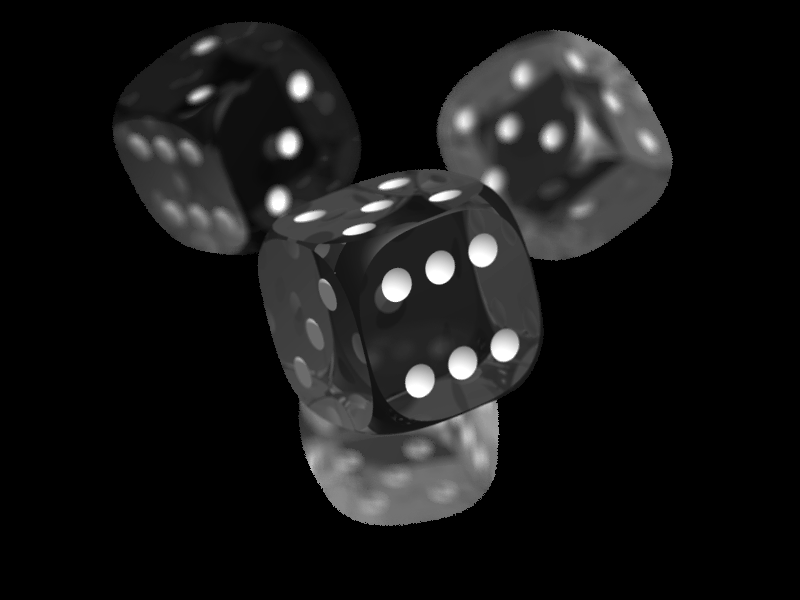
\includegraphics[width=0.20\textwidth]{images/cv-grayscale.png}
    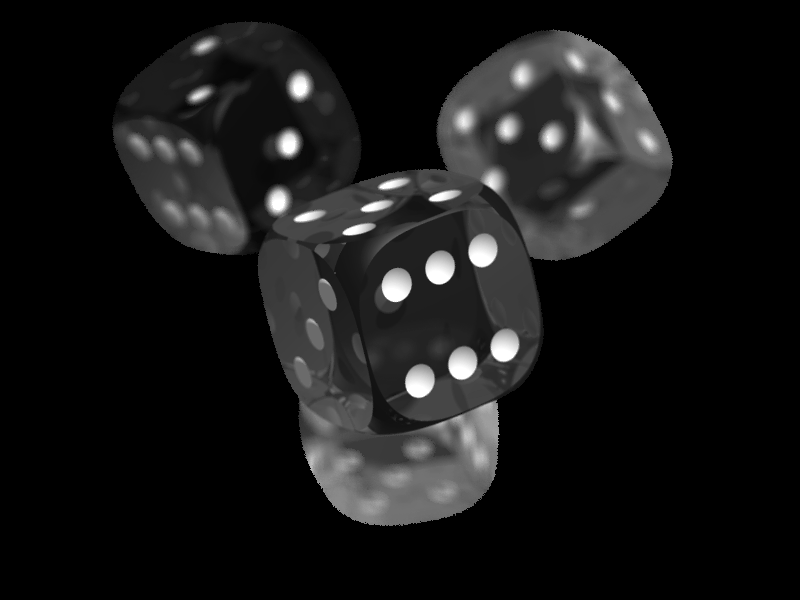
\includegraphics[width=0.20\textwidth]{images/own-grayscale.png}
    
    \caption{Grayscale results of OpenCV (middle) and self-implemented  Algorithm (right)}
    \label{fig:grayscale}
\end{figure}

\section{Implementation}


\begin{listing}[H]
    \begin{minted}{cpp}
cv::Mat applyGrayscaleOuter(cv::Mat srcImage, int numThreads = omp_get_num_procs()) {
    auto destImage = cv::Mat(srcImage.rows, srcImage.cols, CV_8UC1);
    omp_set_num_threads(numThreads);

    #pragma omp parallel for default(none) shared(srcImage, destImage)
    for (int row = 0; row < srcImage.rows; row++) {
        for (int col = 0; col < srcImage.cols; col++) {
            auto srcPixel = srcImage.at<cv::Vec3b>(row, col);

            uchar r = srcPixel[2];
            uchar g = srcPixel[1];
            uchar b = srcPixel[0];

            // uchar destPixel = 0.21 * r + 0.72 * g + 0.07 * b; // luminosity formular
            uchar destPixel = 0.299 * r + 0.587 * g + 0.114 * b; // open cv formular

            destImage.at<uchar>(row, col) = destPixel;
        }
    }

    return destImage;
}
    \end{minted}
    \captionof{lstlisting}{Grayscale with parallelization of the outer For-Loop}
    \label{listing:grayscale}
\end{listing}


\section{Comparison with OpenCV}

\subsection{Code}

Image transformation from color to grayscale can be conveniently done with one line of code in OpenCV.

\begin{listing}[H]
    \begin{minted}{cpp}
cv::cvtColor(srcImage, destImage, cv::COLOR_BGR2GRAY);
    \end{minted}
    \captionof{lstlisting}{Grayscale with OpenCV}
    \label{listing:grayscale_opencv}
\end{listing}

\subsection{Performance}

As OpenCV computes on the GPU with a runtime of $ xxx $, it is significantly faster and outperforms the custom OpenMP.